\begin{tikzpicture}
    \node[anchor=south west,inner sep=2] (realSlurry) at (0,0) {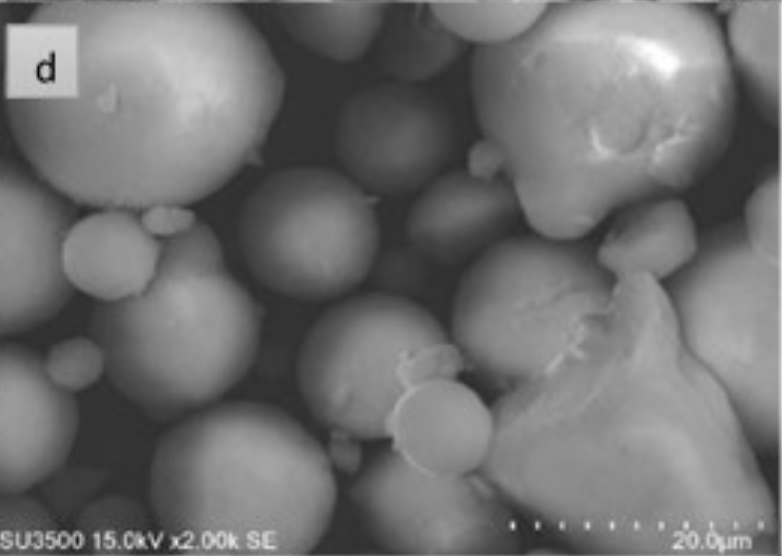
\includegraphics[width=0.3\textwidth]{\myGraphs/washCoating/showCaseParticleDistributionJiankMsTh.png}};
    \node[anchor=north,inner sep=0] (washGreen) at (realSlurry.south) {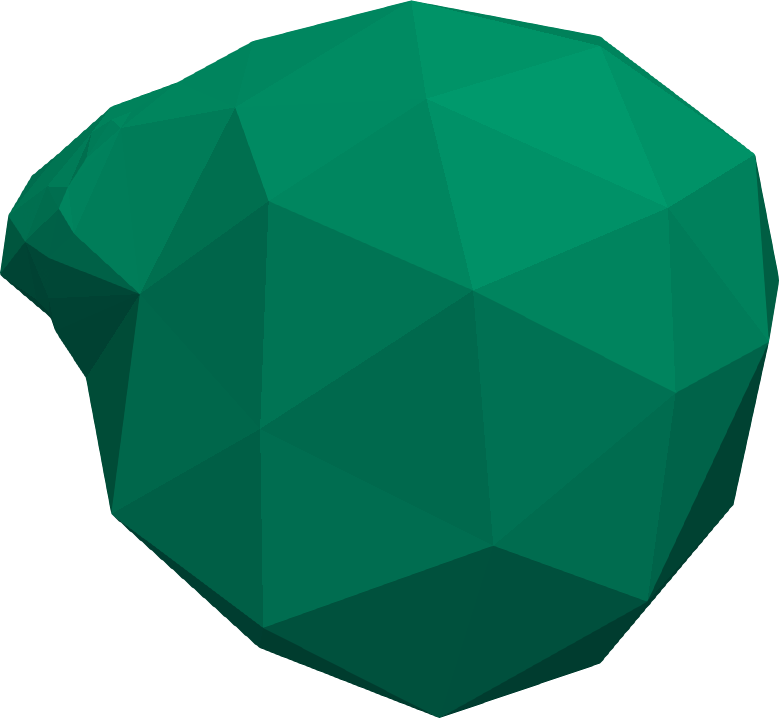
\includegraphics[width=0.25\textwidth]{\myGraphs/washCoating/icoSph_GreenV1.png}};
    \begin{axis}[
        at=(realSlurry.north east),anchor=left of north west,
        name=washDistrib,
        width=0.6\textwidth,
        xshift=0.03\textwidth,
        xlabel={particle diameter $[\mu\mathrm{m}]$},
        ylabel={$q\, [\%]$},
        smooth,
        ymin=0,
        ymax=15,
        xmode=log,
        xmin=1,
        xmax=100,
    ]
    \addplot [color=blue,mark=none,thick] table [x={diameter}, y={avg}] {\myGraphs/washCoating/partSizeDistribV1.dat};
    \draw [dashed,color=black] (axis cs: 3.905,0)--(axis cs:3.905,15) node[pos=0.99,above,rotate=90,font=\small,anchor=south east]{mesh induced cut-off};
    \end{axis}
    \node[anchor=north east] at (realSlurry.north west) {(a)};
    \node[anchor=north east] at (washGreen.north west) {(b)};
    \node[anchor=north east,xshift=-0.05\textwidth] at (washDistrib.north west) {(c)};
\end{tikzpicture}
